\documentclass{article}
\usepackage{tikz}
\usetikzlibrary{arrows.meta, positioning}

\begin{document}

\section{Workflow diagram}

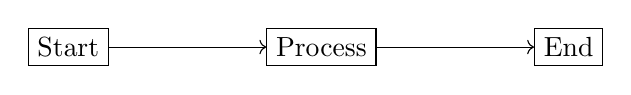
\begin{tikzpicture}[node distance=2cm, auto]
  \node (start) [rectangle, draw] {Start};
  \node (process) [rectangle, draw, right=of start] {Process};
  \node (end) [rectangle, draw, right=of process] {End};
  \draw[->] (start) -- (process);
  \draw[->] (process) -- (end);
\end{tikzpicture}

\section{Plot}

\begin{tikzpicture}
  \draw[->] (-0.5,0) -- (3,0) node[right] {$x$};
  \draw[->] (0,-0.5) -- (0,3) node[above] {$y$};
  \draw[thick,blue] (0,0) parabola (2,2);
\end{tikzpicture}

\end{document}
